\subsection{EXPORTAÇÃO DE GRADES HORÁRIAS}

Considerando a necessidade de exportar as grades horárias para fora do sistema, e a sua natureza tabular, implementou-se a funcionalidade de \textit{download} das grades como planilhas Excel, no formato XLSX.

Para possibilitar a exportação neste formato, utilizou-se o pacote \textit{Node ExcelJs}, que providencia a classe "WorkBook", a qual facilita a construção de arquivos de planilhas Excel utilizando a linguagem \textit{JavaScript}. O resultado final desta implementação pode ser visto na \autoref{fig:gradeExportada}.

\begin{figure}[!htb]
	\centering
	\caption{Grade horária exportada para planilha}
	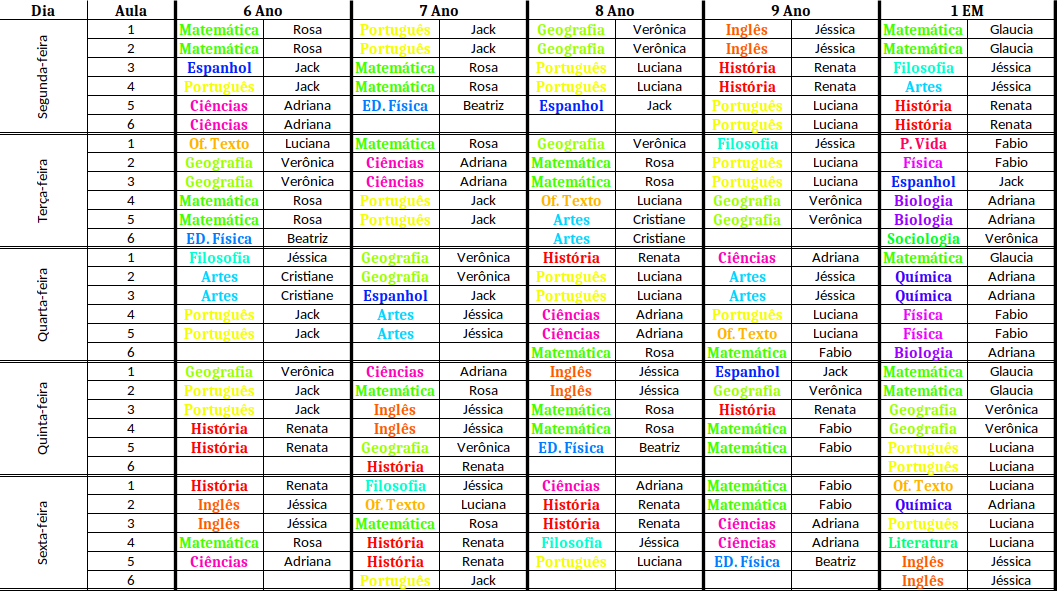
\includegraphics[width=1\textwidth]{./dados/figuras/gradeExportada}
	\fonte{Autor}
	\label{fig:gradeExportada}
\end{figure}

O desenvolvimento deste incremento também involveu a adição de um botão para efetivamente exportar a grade horária, como pode ser visto na \autoref{fig:botaoBaixar}.

\begin{figure}[!htb]
	\centering
	\caption{Botão para exportar grade horária}
	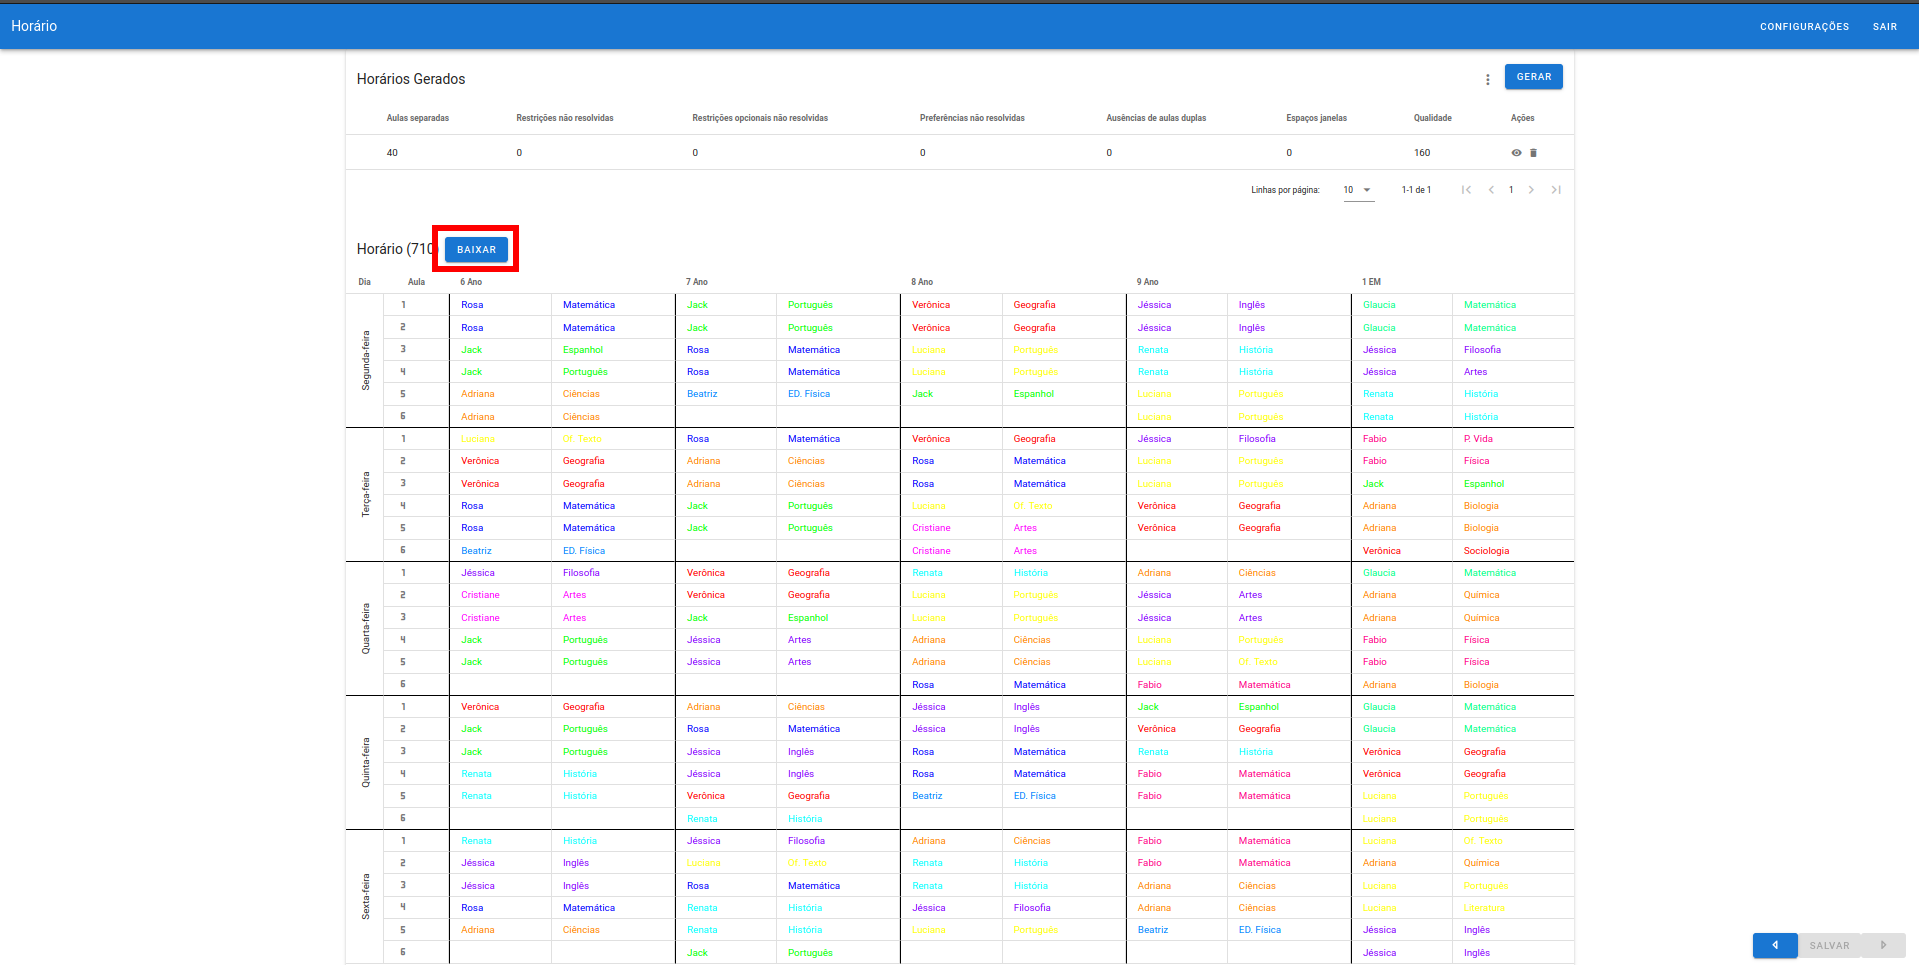
\includegraphics[width=1\textwidth]{./dados/figuras/botaoBaixar}
	\fonte{Autor}
	\label{fig:botaoBaixar}
\end{figure}